\setcounter{problem}{0}

\title{Dynamical Systems \\ Homework 2}
\date{May 19, 2023}

\maketitle

\begin{problem}
~
\begin{enumerate}[a)]
    \item Let \(f \colon \symbb{S}^1 \to \symbb{S}^1\) be a homeomorphism of the unit circle. 

    Fix \(\varepsilon > 0\) and set \(\delta_{\varepsilon} = \ceil{\frac{1}{\varepsilon}}\). Denote by \(E_0\) the set
    \[
        E_0 = \Set{ 0, \frac{1}{\delta_{\varepsilon}}, \dots, \frac{\delta_{\varepsilon} - 1}{\delta_{\varepsilon}} }
    \]
    This is clearly a \(\left(0, \varepsilon\right)\)-spanning set. For any \(n \in \naturals\), define
    \[
        E_n = \bigcup_{k = 0}^{n - 1} \, f^{-k} \left(E_0\right)
    \]
    We claim that this is an \(\left(n, \varepsilon\right)\)-spanning set for \(\symbb{S}^1\). In other words, for any \(x \in \symbb{S}^1\) there exists a \(y \in E_n\) for which \(d_n (x, y) < \varepsilon\).
    
    Assume the contrary, i.e.\ that there exists an \(x \in \symbb{S}^1\) with \(d_n (x, y) \geq \varepsilon\) for any \(y \in E_n\). Let \(z \in E_n\) be the point closest to \(x\) with respect to this distance. There are at most two points with this property, in which case \(x\) is equidistant to them and we can pick either of them for the purpose of our argument.
    
    By definition,
    \[
        d_n (x, z) = \max_{0 \leq k \leq n - 1} d \left(\, f^k(x), \, f^k(z)\right)
    \]
    hence there must be some \(k \in \Set{0, \dots, n - 1}\) for which
    \[
        d\left(\, f^k (x), \, f^k (z)\right) \geq \varepsilon
    \]
    This means that we can fit an open ball of radius \(\varepsilon\) (with respect to the distance \(d\)) between \(f^k (x)\) and \(f^k (z)\). But since \(E_0\) is a \(\left(0, \varepsilon\right)\)-spanning set, there exists some \(t \in E_0\) which is also contained in the interval \(\left(\, f^n (x), \, f^n (z)\right)\) (we've assumed without loss of generality that \(f^n (x) < f^n(z)\), otherwise the endpoints of the interval should be flipped).
    
    Since \(f\) is a homeomorphism, \(f^k\) is as well, so the interval \((x, z)\) gets mapped to \(\left(\, f^k(x), \, f^k(z)\right)\) (again, with the endpoints possibly reversed). In particular, since \(t \in \left(\, f^k(x), \, f^k(z)\right)\), we get \(f^{-k} (t) \subset (x, y)\). This means that some preimage of \(t\), say \(t' \in f^{-k} \left(E_0\right) \subseteq E_n\), is closer to \(x\) than \(y\), a contradiction with our assumption that \(y\) was the point of \(E_n\) closest to \(x\). Hence, we can take \(E_n\) as an \(\left(n, \varepsilon\right)\)-spanning set and use it as an upper bound for the cardinality of a minimal spanning set.

    An estimate for the size of \(E_n\) is
    \[
        \abs{E_n} = \abs{\bigcup_{k = 0}^{n - 1} f^{-k} \left(E_0\right)} \leq \sum_{k = 0}^{n - 1} \abs{\, f^{-k} (E_0)} \leq \sum_{k = 0}^{n - 1} \abs{E_0} = n \, \abs{E_0} = n \cdot \delta_{\varepsilon}
    \]
    so the cardinality of a minimal \(\left(n, \varepsilon\right)\)-spanning set is at most \(n \cdot \delta_{\varepsilon}\). Thus,
    \begin{align*}
        h_{\text{top}} \left(\, f\right) &\leq \lim_{\varepsilon \to 0^{+}} \lim_{n \to \infty} \frac{1}{n} \log \left(n \cdot \delta_{\varepsilon}\right) \\
        &= \lim_{\varepsilon \to 0^{+}} \lim_{n \to \infty} \left(\frac{\log n}{n} + \frac{\log \delta_{\varepsilon}}{n}\right) \\
        &= \lim_{\varepsilon \to 0^{+}} 0 = 0
    \end{align*}

    \item Notice that
    \begin{gather*}
        f(\theta + 1) = (\theta + 1) + \epsilon \sin (2 \pi N (\theta + 1)) \\
        \overset{\Mod{1}}{\resizebox{\widthof{\(\Mod{1}\)}}{\height}{\(\equiv\)}}
        \theta + \epsilon \sin (2 \pi N \theta) = f(\theta)
    \end{gather*}
    hence \(f\) admits a lift \(F \colon \reals \to \reals\), given by
    \[
        F(x) = x + \epsilon \sin (2 \pi N x)
    \]
    If we can show that \(F\) is a homeomorphism, then \(f\) will be as well.

    \begin{itemize}
        \item We remark that \(F\) is in \(\symcal{C}^{\infty} \left(\reals\right)\). Its derivative is
        \[
            F'(x) = 1 + \epsilon \cdot 2 \pi N \cdot \cos (2 \pi N x)
        \]
        Since \(0 < \epsilon < \frac{1}{2 \pi N}\), we get \(0 < \epsilon \cdot 2 \pi N < 1\), whence
        \[
            \abs{\epsilon \cdot 2 \pi N \cdot \cos (2 \pi N x)} < 1
        \]
        which ensures that \(F' (x) > 0\), \(\forall x \in \reals\). This shows that \(F\) is strictly increasing, hence also injective.

        \item Since the \(\epsilon \sin(2 \pi N x)\) term is bounded, we have
        \[
            \lim_{x \to \pm\infty} F(x) = \lim_{x \to \pm \infty} x = \pm \infty
        \]
        which shows that \(F\) is surjective.

        \item Since \(F\) is bijective and differentiable, its inverse is also differentiable (in particular, continuous). Hence \(F\) is a homeomorphism.
    \end{itemize}

    The rotation number of this circle homeomorphism is
    \[
        \rho(F) = \lim_{n \to \infty} \frac{F^{\circ n} (x) - x}{n}
    \]
    which we can rewrite as
    \begin{align*}
        \rho(F) &= \lim_{n \to \infty} \frac{x + \epsilon \sin(2 \pi N \cdot F^{\circ (n - 1)} (x)) - x}{n} \\
        &= \lim_{n \to \infty} \frac{\epsilon \sin(\, \dots)}{n}
    \end{align*}
    Hence, the rotation number of \(F\) is \(\rho(F) = 0\).

    The phase diagram of this function for \(N = 3\) and \(\epsilon = 0.05 < \frac{1}{6 \pi}\) is portrayed in the figure below.
    \begin{figure}[htbp]
        \centering
        \begin{tikzpicture}[
                declare function={
                    func(\x) = \x + 0.05 * sin(deg(2 * pi * 3 * \x))
                ;
              }
            ]
            
            \begin{axis}[
                axis x line=middle, axis y line=middle,
                ymin=0, ymax=1.5, ytick={0,0.2,...,1}, ylabel=$y$,
                xmin=0, xmax=1.5, xtick={0,0.2,...,1}, xlabel=$x$,
                domain=0:1, samples=200
            ]
                \draw[dashed] (axis cs:0, 1) -- (axis cs:1, 1);
                \draw[dashed] (axis cs:1, 0) -- (axis cs:1, 1);
                \draw[dashed] (axis cs:0, 0) -- (axis cs:1, 1);
    
                \addplot [blue,thick] {func(x)};
            \end{axis}
        \end{tikzpicture}
    \end{figure}

    \item The continued fraction expansion of \(\alpha\) is
    \[
        \alpha = [2; 4, 4, \dots] = 2 + \frac{1}{4 + \frac{1}{4 + \dots}}
    \]
    Denoting the term \(\frac{1}{4 + \dots}\) by \(x\), we must have
    \[
        \frac{1}{4 + x} = x
    \]
    whence
    \[
        x^2 + 4x - 1 = 0
    \]
    which has roots \(-2 \pm \sqrt{5}\). Clearly, \(x > 0\), so the only admissible solution is \(x = -2 + \sqrt{5}\). We get that \(\alpha = 2 + x = \sqrt{5}\).

    We claim that \(\sqrt{5}\) is a Brjuno number. Let \(p_n / q_n\) be the \(n\)th rational approximant of \(\sqrt{5}\). Then a \href{https://en.wikipedia.org/wiki/Continued_fraction#Some_useful_theorems}{recurrence formula} for \(q_n\) states that
    \begin{align*}
        q_n &= a_n q_{n - 1} + q_{n - 2} & q_{-1} &= 1 & q_{-2} = 0
    \end{align*}
    where \(a_n\) is the \(n\)th term of the continued fraction expansion of \(\sqrt{5}\). In our case,
    \[
        q_n = 4 q_{n - 1} + q_{n - 2}
    \]
    for \(n \geq 1\). The first few terms are \(q_0 = 2\), \(q_1 = 9\), \(q_2 = 38\), \(q_3 = 161\), \(\dots\). Using the recurrence formula above, it's easy to see that the sequence is bounded between \(3^n\) and \(5^{n + 1}\).
    
    The condition for \(\sqrt{5}\) to be Brjuno is
    \[
        \sum_{n = 1}^{\infty} \frac{\log \left(q_{n + 1}\right)}{q_n} < \infty
    \]
    Replacing with upper and lower bounds, it's enough to check that
    \[
        \sum_{n = 1}^{\infty} \frac{\log \left(5^{n + 2}\right)}{3^n} = \sum_{n = 1}^{\infty} \frac{(n + 2) \cdot \log 5}{3^n} = (\log 5) \cdot \sum_{n = 1}^{\infty} \frac{n + 2}{3^n} < \infty
    \]
    The series on the right is clearly convergent.
    
    Hence, \(\sqrt{5}\) is Brjuno, and a theorem from the course tells us that \(p(z)\) is locally (on the boundary of the Siegel disk) conjugate with the irrational rotation \(z \mapsto \lambda z\), where \(\lambda = e^{2 \pi i \sqrt{5}}\). In particular, we have \(\rho(p) = \sqrt{5}\).
\end{enumerate}
\end{problem}

\begin{problem}
~
\begin{enumerate}[a)]
    \item A point \(z \in \complex\) is a fixed point for \(p_c\) if
    \begin{align*}
        &p_c (z) = z \\
        \iff
        &z^2 + c = z \\
        \iff
        &z^2 - z + c = 0
    \end{align*}
    which has discriminant \(\Delta = 1 - 4 c\) and roots \(z = \frac{1 \pm \sqrt{\Delta}}{2}\). A fixed point \(z\) is attracting or indifferent if
    \begin{align*}
        &\abs{p'_c (z)} \leq 1 \\
        \iff
        &\abs{2 \cdot z} \leq 1 \\
        \iff
        &\abs{2 \cdot \frac{1 \pm \sqrt{\Delta}}{2}} \leq 1 \\
        \iff
        &\abs{1 \pm \sqrt{1 - 4c}} \leq 1
    \end{align*}
    The boundary of this region is given by
    \[
        \abs{1 \pm \sqrt{1 - 4c}} = 1    
    \]
    Since \(2 \abs{z} = 1\), we have \(z = e^{i t} /2 \) for some \(t \in \reals\). Plugging this back into the original polynomial, we have
    \[
        z - z^2 = c \iff \frac{e^{i t}}{2} - \frac{e^{2 i t}}{4} = c
    \]
    or explicitly, using Euler's formula and writing \(c = x + i y\), we obtain
    \begin{gather*}
        \frac{\cos t + i \sin t}{2} - \frac{\cos 2t + i \sin 2t}{4} = x + iy \\
        \iff
        2 \cos t - \cos 2t + 2 i \sin t - i \sin 2t = 4 x + 4 i y \\
        \iff
        \begin{cases}
            x = \frac{1}{4} (2 \cos t - \cos 2t) \\
            y = \frac{1}{4} (2 \sin t - \sin 2t)
        \end{cases}
    \end{gather*}
    
    This cardioid is plotted in the figure below.
    
    \begin{figure}[htbp]
        \centering
        \begin{tikzpicture}            
            \begin{axis}[
                axis x line=middle, axis y line=middle,
                ymin=-1, ymax=1, ytick={-1,...,1}, ylabel=$y$,
                xmin=-1, xmax=1, xtick={-1,...,1}, xlabel=$x$,
                trig format plots=rad,
                variable=t
            ]          
                \addplot[blue,thick,domain=0:2*pi,samples=200]
                ({0.25 * (2 * cos(t) - cos(2 * t))}, {0.25 * (2 * sin(t) - sin(2 * t)))});
            \end{axis}
        \end{tikzpicture}
    \end{figure}

    \item A point \(z \in \complex\) is periodic with period (at most) two if the following equation holds:
    \begin{gather*}
        p_c \left(\, p_c (z)\right) = z \\
        \iff
        (z^2 + c)^2 + c = z \\
        \iff
        z^4 + 2 c z^2 + c^2 + c = z \\
        \iff
        c^2 + c(2 z^2 + 1) + (z^4 - z) = 0
    \end{gather*}
    Solving for \(c\), we have
    \begin{align*}
        \Delta &= (2 z^2 + 1)^2 - 4 (z^4 - z) \\
        &= 4 z^4 + 4 z^2 + 1 - 4 z^4 + 4 z \\
        &= 4 z^2 + 4 z + 1 \\
        &= (2 z + 1)^2
    \end{align*}
    and
    \begin{gather*}
        c_{1, 2} = \frac{- 2z^2 - 1 \pm (2z + 1)}{2} \\
        \implies \begin{cases}
            c_1 = - z^2 + z \\
            c_2 = - z^2 - z - 1
        \end{cases}
    \end{gather*}
    The first family of solutions gives us the periodic points of period 1 (the fixed points), as we've seen previously. We will be interested in finding the values of \(c\) associated with the second solution.
    
    Let us now also impose the attracting or indifferent periodic point condition,
    \begin{gather*}
        \abs{(p_c \circ p_c)' (z)} \leq 1 \\
        \iff
        \abs{\left(\left(z^2 + c\right)^2 + c\right)'} \leq 1 \\
        \iff
        \abs{4 z (z^2 + c)} \leq 1
    \end{gather*}
    and the boundary of this region is
    \[
        4 \abs{z (z^2 + c)} = 1 \iff z (z^2 + c) = \frac{e^{i t}}{4}
    \]
    Substituting the solution \(c_2\) into this equation, we obtain
    \begin{gather*}
        z (z^2 - z^2 - z - 1) = \frac{e^{it}}{4} \\
        \iff
        z (-z - 1) = \frac{e^{it}}{4} \\
        \iff
        z^2 + z = -\frac{e^{it}}{4}
    \end{gather*}
    But now using the fact that \(z^2 + z + 1 = -c\), we can deduce
    \[
        - c - 1 = - \frac{e^it}{4}
    \]
    whence
    \[
        c = \frac{e^{it}}{4} - 1
    \]
    The corresponding parametrization is
    \[
        \begin{cases}
            x = \frac{1}{4} \cos t - 1 \\
            y = \frac{1}{4} \sin t
        \end{cases}
    \]
    i.e. a circle of radius \(\frac{1}{4}\) centered at the point \((-1, 0)\).

    The figure below shows both the main cardioid and the circular region we've determined.

    \begin{figure}[htbp]
        \centering
        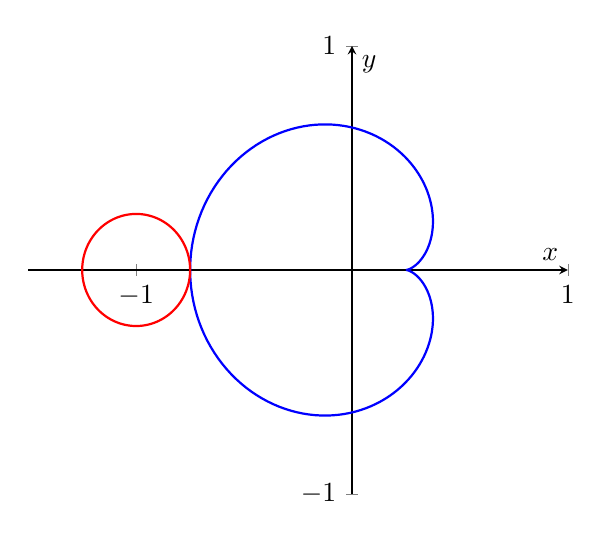
\begin{tikzpicture}            
            \begin{axis}[
                axis x line=middle, axis y line=middle,
                ymin=-1, ymax=1, ytick={-1,...,1}, ylabel=$y$,
                xmin=-1.5, xmax=1, xtick={-1,...,1}, xlabel=$x$,
                trig format plots=rad,
                variable=t
            ]
                \addplot[blue,thick,domain=0:2*pi,samples=200]
                ({0.25 * (2 * cos(t) - cos(2 * t))}, {0.25 * (2 * sin(t) - sin(2 * t)))});
                
                \addplot[red,thick,domain=0:2*pi,samples=200]
                ({0.25 * cos(t) - 1}, {0.25 * sin(t)});
            \end{axis}
        \end{tikzpicture}
    \end{figure}

    \item An intersection point of \(R\) and \(C\) is at \(c = -\frac{3}{4}\). We are going to show that this point is not structurally stable.
    
    Let \(\varepsilon > 0\) be a small positive real number. If we take \(\delta = -\varepsilon\), then \(c - \varepsilon\) will land in the hyperbolic component of the Mandelbrot set where the polynomials have attracting cycles of period 2. If we take \(\delta = +\varepsilon\), then \(c + \varepsilon\) will land in the hyperbolic component of the Mandelbrot set where the polynomials have an attracting fixed point. Hence, these two kinds of polynomials cannot be topologically conjugate on their corresponding Julia sets.
\end{enumerate}
\end{problem}

\begin{problem}
Let \(\gamma = \left(\gamma_1, \dots, \gamma_n\right)\) be a point in \(\torus^n\) such that \(1, \gamma_1, \dots, \gamma_n\) are rationally independent (linearly independent over \(\rationals\)). Let \(f \colon \torus^n \to \torus^n\) be given by
\[
    f\left(x_1, \dots, x_n\right) = \left(x_1 + \gamma_1, \dots, x_n + \gamma_n\right) \, \symrm{mod} \, 1
\]
We will show that \(f\) is ergodic with respect to the Lebesgue measure \(\lambda\) using a proof by contradiction. Suppose that there exists \(g \in L^2 (\torus^n, \lambda)\) such that
\[
    g \circ f = g
\]
for \(\lambda\)-almost every point.

Decompose \(g\) as a multidimensional Fourier series,
\[
    g (x) = \sum_{k_1 = -\infty}^{+\infty} \cdots \sum_{k_n = -\infty}^{+\infty} c_{k_1 \dots k_n} \, e^{2 \pi i (k \cdot x)}
\]
where we've denoted by \(k \cdot x\) the dot product between the vectors \(k = \left(k_1, \dots, k_n\right)\) and \(x = \left(x_1, \dots, x_n\right)\). Then the Fourier series of \(g \circ f\) will be equal to
\[
    (g \circ f) (x) = \sum_{k_1 = -\infty}^{+\infty} \cdots \sum_{k_n = -\infty}^{+\infty} c_{k_1 \dots k_n} \, e^{2 \pi i (k \cdot \gamma)} \, e^{2 \pi i (k \cdot x)}
\]
The Fourier series decomposition is unique, therefore we must have
\[
    c_{k_1 \dots k_n} = c_{k_1 \dots k_n} e^{2 \pi i (k \cdot \gamma)} = c_{k_1 \dots k_n} e^{2 \pi i (k_1 \gamma_1 + \dots + k_n \gamma_n)}
\]
for all \(k = \left(k_1, \dots, k_n\right) \in \integers^n\). For \(k \neq 0\), assuming \(c_{k_1 \dots k_n} \neq 0\), the equality holds only if
\[
    k_1 \gamma_1 + \dots + k_n \gamma_n = 0
\]
Since \(\gamma_1, \dots, \gamma_n\) are linearly independent over \(\rationals\), a result from linear algebra lets us conclude that they are linearly independent over \(\integers\) as well. Hence the only possibility is \(c_{k_1 \dots k_n} = 0\) whenever \(k \neq 0\). In other words, the only non-zero Fourier coefficient of \(g\) is \(c_0\). This forces \(g\) to be a constant (\(\lambda\)-almost everywhere), which shows that \(f\) is ergodic.

Finally, we remark that \(\torus^n\) is a compact metric space and a topological group at the same time, with \(\lambda\) being the corresponding Haar measure. By a theorem from the course, this lets us conclude that the translation determined by \(\gamma\) is uniquely ergodic.

\begin{comment}
To show that it is uniquely ergodic, we will use a theorem due to Furstenberg, from his paper ``\href{https://www.jstor.org/stable/2372899}{Strict Ergodicity and Transformation of the Torus}'':

Let \(T\) be a continuous transformation of a compact metric space \(X\) and \(\varphi \colon X \to \torus\) a continuous function. Define the transformation \(\hat{T}\) on \(\hat{X} \coloneq X \times \torus\) by
\[
    \hat{T} (x, t) = \left(T(x), t + \varphi(x)\right)
\]
Let \(\mu\) be the unique \(T\)-invariant measure on \(X\). Denote by \(\hat{\mu}\) the product measure \(\mu \otimes \lambda\). If \(\hat{\mu}\) is \(\hat{T}\)-ergodic, then it is uniquely ergodic.

We will reproduce a proof of this statement, as presented \href{http://homepages.math.uic.edu/~furman/preprints/intro-ET.pdf}{here}. Suppose that we know that \(\mu\) is the unique \(T\)-invariant measure on \(X\) and \(\hat{\mu} = \mu \otimes \lambda\) is \(\hat{T}\)-ergodic. Let \(\hat{\nu}_0\) be some invariant measure for \(\hat{T}\). Define \(\hat{\nu}_t\) be the translation by \(t \in \torus\) of \(\hat{\nu}\), i.e.
\[
    \int_{\hat{X}} f(x, s) \diff \hat{\nu}_t (x, s) = \int_{\hat{X}} f(x, s + t) \diff \hat{\nu}_0 (x, s)
\]
for any continuous \(f \colon \hat{X} \to \reals\). Since \(\hat{\nu}_0\) is \(\hat{T}\)-invariant, \(\hat{\nu}_t\) is as well.

We can also define the ``average'' measure \(\bar{\nu}\) as
\begin{align*}
    \int_{\hat{X}} \, f(x, s) \diff \bar{\nu} (x, s) &= \int_{\torus} \left(\int_{\hat{X}} f(x, s) \diff \hat{\nu}_t (x, s)\right) \diff t \\
    &= \int_{\torus} \left(\int_{\hat{X}} f(x, s + t) \diff \hat{\nu}_0 (x, s) \right) \diff t \\
    &= \int_{\hat{X}} \left(\int_{\torus} f(x, s + t) \diff t\right) \diff \hat{\nu}_0 (x, s) \\
    &= \int_{\hat{X}} \left(\int_{\torus} f(x, t) \diff t\right) \diff \hat{\nu}_0 (x, s) \\
    &= \int_{\hat{X}} \, f (x, s) \diff (p^* \hat{\nu}_0 \otimes \lambda) (x, s)
\end{align*}
where we've used Fubini's theorem to switch the order of integration and denoted by \(p^* \hat{\nu}_0\) the push-forward of the measure \(\hat{\nu}_0\) through the projection \(p \colon \hat{X} \to X\). By construction, \(p^* \hat{\nu}_0\) is \(T\)-invariant. But since \(\mu\) is the unique \(T\)-invariant measure on \(X\) by hypothesis, we get that \(p^* \hat{\nu}_0 = \mu\). Hence
\[
    \int_{\Hat{X}} f(x, s) \diff \bar{\nu} (x, s) = \int_{\hat{X}} f(x, s) \diff \hat{\mu} (x, s)
\]

By an analogous computation, we can obtain \(p^* \hat{\nu}_1 = \mu\). 
We also know from the hypothesis that \(\hat{\mu}\) is \(\hat{T}\)-ergodic, hence an extremal point in the space of \(\hat{T}\)-invariant measures. This shows that \(\hat{\nu}_t = \mu \otimes \lambda\) for almost all \(t\). In particular, reversing the translation on \(\hat{\nu}_s\) for some \(s \in \torus\) for which this equality holds, we obtain that \(\hat{\nu}_0 = \mu \otimes \lambda = \hat{\mu}\). Since \(\hat{\nu}_0\) was chosen arbitrarily, we can conclude that \(\hat{\mu}\) is the unique \(\hat{T}\)-ergodic measure on \(\hat{X}\).

We can use this theorem to prove the unique ergodicity of an irrational rotation on the \(n\)-torus by induction. For the base case, take \(X\) to be a point, \(\mu\) to be the Dirac measure centered on this point, \(T\) to be the identity map and \(\varphi (x) = \gamma_1\). For the induction step, write \(\torus^k = \torus^{k - 1} \times \torus\) and define \(\varphi_k (x) = \gamma_k\). We get that
\[
    \hat{T} (x, t) = \left(x_{1 \dots k - 1} + \gamma_{1 \dots k - 1}, t + \gamma_{k}\right)
\]
is uniquely ergodic with respect to \(\lambda^k = \lambda^{k - 1} \otimes \lambda\).
\end{comment}
\end{problem}

\begin{problem}
~
\begin{enumerate}[a)]
    \item Let \(\mu_1 \neq \mu_2\) be two ergodic measures for a continuous map \(T \colon X \to X\) on a compact metric space \(X\).
    
    We will first prove that neither of the measures can be absolutely continuous with respect to the other. Recall that \(\mu_1\) is absolutely continuous with respect to \(\mu_2\), a relation we will denote by \(\mu_1 \ll \mu_2\), if \(\mu_2(A) = 0\) implies \(\mu_1(A) = 0\) for any measurable set \(A\).

    Suppose that \(\mu_1 \ll \mu_2\). Let \(\varphi \colon X \to \reals\) be any bounded measurable function. Clearly, it is Lebesgue integrable with respect to our measures. By Birkhoff's ergodic theorem, we have
    \[
        \lim_{n \to \infty} \frac{1}{n} \varphi(T^n (x)) = \int_{X} \varphi \diff \mu_2
    \]
    for almost every \(x \in X\), i.e.\ for every \(x\) in some subset \(A\) with \(\mu_2 (A) = 1\). Furthermore, we have \(\mu_2 (X \setminus A) = 1 - \mu_2 (A) = 0\). Since we've assumed that \(\mu_1 \ll \mu_2\), this implies \(\mu_1 (X \setminus A) = 0\), whence \(\mu_1 (A) = 1\) as well. Applying Birkhoff's ergodic theorem again we obtain
    \[
        \lim_{n \to \infty} \frac{1}{n} \varphi(T^n (x)) = \int_X \varphi \diff \mu_1
    \]
    for all \(x \in A\), hence
    \[
        \int_{X} \varphi \diff \mu_1 = \int_X \varphi \diff \mu_2
    \]
    The choice of \(\varphi\) was arbitrary. Taking the characteristic functions of any measurable subset \(Y\) of \(X\), we get a contradiction with the fact that \(\mu_1 \neq \mu_2\). Hence, \(\mu_1\) is not absolutely continuous with respect to \(\mu_2\). We get the corresponding conclusion for absolute continuity of \(\mu_2\) with respect to \(\mu_1\) by symmetry.

    Negating the definition of absolute continuity, we can deduce that there exists some measurable set \(S \subseteq X\) for which \(\mu_2 (S) = 0\), yet \(\mu_1 (S) > 0\). Define the set \(A\) by
    \[
        A = \limsup_{k \to \infty} {T^{-k} (S)} = \bigcap_{i \, = \, 0}^{+\infty} \bigcup_{j \, = \, i}^{+\infty} T^{-j} (S)
    \]
    A point \(x\) is in \(A\) iff there exists an \(s \in S\) such that \(x \in T^{-k} (s)\) for infinitely many values of \(k\). This shows that \(T^{-1} (x)\) is also in \(A\), hence \(A\) is \(T\)-invariant.

    We will show that \(\mu_1 (A) = 1\) and \(\mu_2 (A) = 0\). Letting \(B \coloneq X \setminus A\), we will get that \(\mu_2 (B) = 1\), which implies that \(\mu_1\) and \(\mu_2\) are mutually singular.

    First, by monotonicity,
    \[
        \mu_1 \left(\, \bigcup_{k \, = \, 0}^{+\infty} T^{-k} (S)\right) \geq \mu_1 \left(T^{-j} (S)\right), \forall j \in \naturals
    \]
    and using the fact that \(\mu_1\) is \(T\)-invariant, we obtain
    \[
        \mu_1 (T^{-j} (S)) = \mu_1 (S) > 0, \forall j \in \naturals
    \]
    Even more,
    \[
        \mu_1 \left(\, \bigcup_{j \, = \, i}^{+\infty} T^{-j} (S)\right) = \mu_1 \left(T^{-i} \left(\bigcup_{k \, = \, 0}^{+\infty} T^{-k} (S)\right)\right) = \mu_1 \left(\bigcup_{k \, = \, 0}^{+\infty} T^{-k} (S)\right)
    \]
    We remark that the sequence of sets \(\bigcup_{j \, = \, i}^{+\infty} \, T^{-j} (S)\) is decreasing, hence
    \begin{align*}
        \mu_1 (A) &= \mu_1 \left(\bigcap_{i \, = \, 0}^{+\infty} \bigcup_{j \, = \, i}^{+\infty} T^{-j} (S)\right) \\
        &= \inf_{i \, \geq \, 0} \, \mu_1 \left(\, \bigcup_{j \, = \, i}^{+\infty} T^{-j} (S)\right) \\
        &= \mu_1 \left(\bigcup_{k \, = \, 0}^{+\infty} T^{-k} (S)\right) > 0
    \end{align*}
    which forces \(\mu_1 (A) = 1\) by ergodicity.

    Analogously, for \(\mu_2\) we get
    \[
        \mu_2 \left(\bigcup_{k \, = \, 0}^{+\infty} T^{-k} (S)\right) \leq \sum_{k \, = \, 0}^{+\infty} \mu_2 \left(T^{-k} (S)\right) = \sum_{k \, = \, 0}^{+\infty} \mu_2 (S) = \sum_{k \, = \, 0}^{+\infty} 0 = 0
    \]
    and
    \[
        \mu_2 \left(\,\bigcup_{j \, = \, i}^{+\infty} T^{-j} (S)\right) = \mu_2 \left(T^{-i} \left(\bigcup_{k \, = \, 0}^{+\infty} T^{-k} (S)\right)\right) = \mu_2 \left(\bigcup_{k \, = \, 0}^{+\infty} T^{-k} (S)\right) = 0
    \]
    whence
    \[
        \mu_2 (A) = \mu_2 \left(\bigcap_{i \, = \, 0}^{+\infty} \bigcup_{j \, = \, i}^{+\infty} T^{-j} (S)\right) = \inf_{i \, \geq \, 0} \mu_2 \left(\bigcup_{j = i}^{+\infty} T^{-j} (S)\right) = 0
    \]
    as claimed.

    % TODO: finish
    \begin{comment}
    \item The support of a measure is defined as
    \[
        \supp \left(\mu\right) = \Set{ x \in X | \mu(U) > 0, \forall U \text{ open neighborhood of } x }
    \]

    Let \(U\) and \(V\) be two non-empty open sets of \(\supp (\mu)\). To show that \(\left.T\right|_{\supp\left(\mu\right)}\) is topologically transitive, we need to show that there exists an \(n\) such that
    \[
        T^n (U) \cap V \neq 0
    \]
    Since \(U\) and \(V\) are not the empty set, each contains a point \(x\), respectively \(y\), of \(\supp\left(\mu\right)\). Let us suppose that \(x \neq y\), since otherwise there is nothing to show.
    \end{comment}
\end{enumerate}
\end{problem}